%\section*{Introduction}
%\addcontentsline{toc}{section}{Introduction}

Le projet présent est effectué au sein de \textquote{Djagora Academy} dans un
équipe des étudiants. Dans la partie qui suit, on va présenter l'organisme
d'accueil \textquote{Djagora Academy}, l'équipe de travail et le sujet du
projet. Ainsi que la méthodologie de gestion du projet choisi.


\section{Organisme d'accueil \textquote{Djagora Academy}}

\begin{figure}[!h]
    \centering
    
\includegraphics[width=.35\textwidth]{logo-djagora}
    \caption{Logo du \textquote{Djagora Academy}}
    \label{fig:logo-djagora}
\end{figure}

\textquote{Djagora Academy} est un programme de mentorat visant accompagner des
étudiants en année terminale dans la réalisation de projets d'intérêt publique
dans le but est la création des startups.

Pendant la réalisation des projets des idées des startups, les étudiants
(mentorés) seront accompagnés par des universitaires et des industriels
(mentors) avec le soutien de plusieurs compagnies internationales, telles que
l'European Center for Leadership and Entrepreneurship Education (Eclee France,
Eclee USA), Djagora University (SénégaL), NorthStar Paradigm Education (USA),
Continental (Allemagne), Sivantos (Allemagne), Yousoft-IT (Tunisie), Factory
Campus (Tunisie).

La première version du \textquote{Djagora Academy}, année 2017, a eu le
lancement de deux idées de startup: \textquote{City Watch} et \textquote{City
Clean}.

\section{Contexte du Projet}

Le projet \textquote{City Watch} consiste à créer un système de logiciel qui
collecte, traite, analyse et visualise des données/informations routières. Il
est composé de trois axes principales:

\begin{enumerate}
    \item Collecte des données là on essaie de résoudre le système adéquat pour
        collecter le maximum de données utiles.
    \item Analyse, filtrage, transformation et exploitation des données.
    \item Valorisation et visualisation des données utiles.
\end{enumerate}

En effet, le mécanisme de collecte est basé sur des applications mobile qui
collectent les données à travers les smartphones et les tablettes et des
applications web qui collectent les données à travers des formulaires. Le
deuxième axe se base sur un système intelligent pour analyser les données
collectées et le troisième axe se base sur un système de visualisation et de
valorisation de ces données en les visualisant sur un matériel cartographique
et préparation de statistiques et de rapports.

Le domaine ciblé de notre projet est le trafic routière comme l'embouteillage,
les accidents, l'infrastructure, \ldots.  Vu la complexité du trois axes, le
projet a été distribué aux membres de l'équipe \textquote{City Watch} pour
atteindre les objectifs tracés. Nous, comme étant un binôme travaillant
collectivement avec les autres membres, nos tâches été plus concentrés sur la
partie de collecte et de stockage des données sur des bases des données bien
structurées.

\section{Objectifs du projet}

L'objectif du projet \textquote{City Watch} est de former une étude de startup
et de créer un système qui vise la centralisation des données qui tournent au
tour le trafic routier. Dans ce cadre, il est impérativement conseillé de
maximiser le nombre des données collectées, de les structurer à fin de les
utilisés convenablement pour fournir des services de consultation pour tous les
intervenants routier par exemple les citoyens, les municipalités, les services
bancaires, les services de sécurité, les sociétés de transport, \ldots.  Tous
intervenants de notre système peuvent être des consommateurs et aussi
fournisseurs de données.

Les donnés sont collectés et envoyés vers le serveur pour les stocker. Puis,
ils seront analysés et visualisés en forme des diagrammes et des cartographiques.
Finalement, ils seront utilisés pour assister l'utilisateur dans la route.
Ces différentes couches sont présentées dans la figure~\ref{fig:citywatch-modules}.

\begin{figure}[!h]
    \centering
    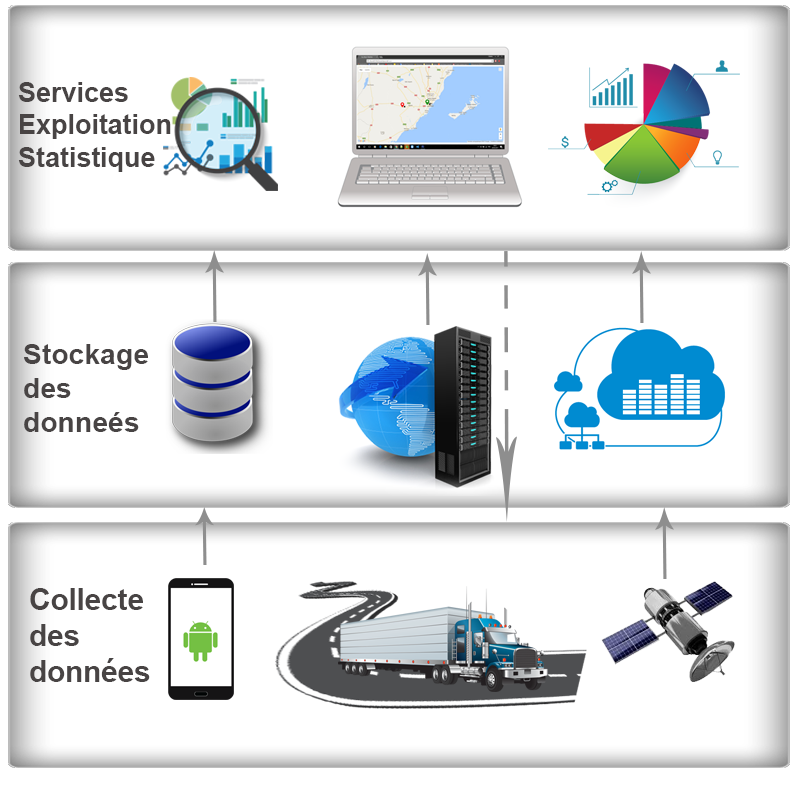
\includegraphics[width=1\textwidth]{citywatch-modules}
    \caption{Vue d'ensemble de la plateforme \textquote{City Watch}}
\label{fig:citywatch-modules}
\end{figure}

\section{Gestion du projet \textquote{City Watch}}

Chaque projet, surtout les projets innovant, doivent cibler une méthodologie
du travail adéquate pour organiser le travail. Parmi les méthodes actuelles, la
plus connue et répondue est la méthode ``Scrum''.

\subsection{Méthodologie agile Scrum}

Scrum est une méthode de gestion de projets dans laquelle des équipes
multifonctionnelles réalisent des produits de manière itérative et
incrémentale. Tout au long de cette méthode, le développement est définit,
d'une façon incrémentale, en cycles de travail appelés Sprints. Un sprint est
définit sous la forme d'un certain nombre de tâches à réaliser au cours d'une
itération. Cette dernière ne dure jamais plus que quatre semaines (deux
semaines la plupart du temps). Les itérations s'enchaînent l'une après l'autre
sans interruption. Les Sprints se terminent à une date spécifique. Ceux-ci ne
peuvent être prolongés même si le travail ne soit pas terminé. Généralement les
équipes Scrum choisissent une durée de Sprint et la maintiennent durant le
projet, jusqu'à ce qu'elles puissent encore augmenter leur productivité et
utiliser alors un cycle plus court. Au début de chaque Sprint, une équipe
multifonctionnelle (environ de quatre à sept personnes) sélectionne des tâches
(exigences du client) dans une liste priorisée. L'équipe s'accorde
collectivement sur une cible constituée de ce qu'elle pense pouvoir livrer à la
fin du Sprint. Aucune nouvelle tâche n'est ajoutée durant le Sprint. Chaque
jour, l'équipe se réunit brièvement afin de contrôler sa progression et ajuster
les prochaines étapes nécessaires à la finalisation du travail restant au sein
d'un Sprint. A la fin de chaque Sprint, une revue est organisée avec les
parties prenantes durant laquelle l'équipe montre ce qu'elle a réalisé. Le
feedback obtenu peut être pris en compte sur le Sprint suivant. Scrum insiste
sur la nécessité de livrer un produit opérationnel, testé et documenté à la fin
de chaque itération. La figure~\ref{fig:scrum-model} représente la méthode
agile Scrum.
%\documentclass{standalone}

%\usepackage{mathpazo}
%\usepackage{tikz}

\usetikzlibrary{calc}
\usetikzlibrary{positioning}
\usetikzlibrary{shapes}

%\begin{document}

\tikzstyle{box} = [rectangle, rounded corners, draw=black, text width=10em, minimum height=3em, text centered]
\begin{figure}[htbp]
  \centering
  \footnotesize
  %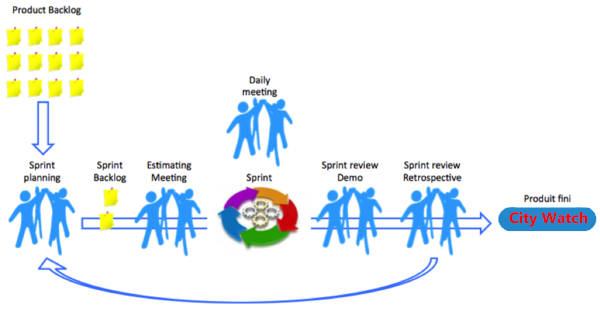
\includegraphics[width=\textwidth]{./figures/scrum-model.tex}
\begin{tikzpicture}

  \node[box]
    (sprints) {Sprints};
  \node[box, left=4em of sprints]
    (planning) {Planning \& System Architecture};
  \node[box, right=4em of sprints]
    (closure) {Closure};

  \draw[->,latex-,line width=0.1em] (5:6em) arc (5:85:6em) node[right=2em] {Wrap};
  \draw[->,latex-,line width=0.1em] (95:6em) node[left=2.5em] {Develop} arc (95:175:6em);
  \draw[->,latex-,line width=0.1em] (185:6em) arc (185:265:6em) node[left=2em] {Adjust};
  \draw[->,latex-,line width=0.1em] (275:6em) node[right=2.5em] {Review} arc (275:355:6em);

  \draw[->,latex-] (planning.west) -- +(-2em,0);
  \draw[->,-latex] (planning.east) to (sprints.west);
  \draw[->,-latex] (sprints.east) to (closure.west);
  \draw[->,-latex] (closure.east) -- +(2em,0);

\end{tikzpicture}
\caption[Méthode Scrum]{La méthode Génie Logiciel Scrum comme décrite par \textcite{Schwaber1995}.}
\captionsource{Daniel G. Siegel, Typical Development Processes of Free and Open Source Software Projects}
\label{fig:scrum-model}
\end{figure}

%\end{document}

L'application de la méthodologie Scrum dans notre projet \textquote{City Watch}
va être plus exploitée et détaillée dans le \autoref{sec:sprint0} ``Itération
0''. Ainsi, la réduction de cet rapport suivi un descriptif appliquant la
méthode Scrum donc le nom des chapitres suivants est basé sur le nom des
itérations Scrum.

\subsection{Justification du choix de la méthode agile Scrum}

Aujourd'hui, La méthodes classique présente beaucoup d'inconvénients:

\begin{itemize}
    \item Parfois le client a du mal à exprimer son besoin. Une telle erreur
        peut s'avérer coûteuse d'autant la modification de certaines
        fonctionnalités dans le projet n'est pas tolérée dans la phase de
        développement. Ce que le nomme l'effet tunnel.
    \item Il est très difficile d'établir dès le début des paramètres stricts
        et clairs qui répondent aux attentes du client.
\end{itemize}

À fin d'éviter ces problèmes, Les caractéristiques de la méthode Scrum offre
des avantages considérables pour gérer ces problèmes:

\begin{description}
    \item [Personnel engagé] L'une des caractéristiques de Scrum, c'est que le
        personnel participe activement à la définition des activités et des
        horaires, de sorte que le degré d'engagement et la motivation sont plus
        élevés.
    \item [Meilleur vue d'ensemble du projet] Avec Scrum, les projets
        précédemment vus dans leur globalité et de façon homogène uniquement
        par les gestionnaires de projets sont désormais accessibles à tous les
        membres de l'équipe de livraison.
    \item [Réduction des bugs] La méthode Scrum privilégie la qualité et la
        fonctionnalité des développements. Le nombre de bugs et de reprises est
        ainsi réduit.
    \item [Mise à jour des priorités] Au début, le client ignore toute la
        portée de l'application, ainsi que la façon dont cela pourrait changer
        avec le temps. Grâce à Scrum, le client bénéficie d'une flexibilité au
        niveau de la définition, de l'évolution des priorités et des séquences
        d'activités.
    \item [Qualité du produit mise en avant] La méthode Scrum se concentre
        davantage sur la fourniture d'un service de valeur au client plutôt que
        sur une date limite fixée.
\end{description}

La nature d'itérations du Scrum et l'engagement des tous les membres concernés
par le projet permettent l'affinement continuel de les quatre variables du
projet, nommées \textquote{Project Diamond} et présentés par la
figure~\ref{fig:project-diamond}:

\begin{description}
    \item [Fonctionnalités] Les cas d'utilisations demandés par le client.
    \item [Ressources] Budget fourni par le client.
    \item [Qualité] Qualité du code à maintenir par l'équipe.
    \item [Estimation] Temps estimé par l'équipe pour la réalisation du code.
\end{description}

\begin{figure}[H]
    \centering
\tikzset{nodes={font=\ttfamily,fill=white}}
\begin{tikzpicture}[
        declare function={%
            f(\t)=90-\t*90;
            g(\t)=\t/2.5+1*\t/(0.1+\t);
            f2(\t)=-90-\t*90;
            g2(\t)=\t/2.5+0.8;
        },
        pos par/.style={%
            shift={({f2(#1)}:{g2(#1)})}
        },
        scale=0.68,
        every node/.style={transform shape},
    ]
    \draw[thick,->] (0,0) -- (0,4.7) node[above]{Fonctionnalités};
    \draw[thick,->] (0,0) -- (4.5,0) node[right]{Resources};
    \draw[thick,->] (0,0) -- (0,-4.5) node[below]{Qualité};
    \draw[thick,->] (0,0) -- (-4.5,0) node[left]{Temps};
    \draw[domain=0:8,variable=\t,smooth,samples=440,arrows={->[length=8]}]
         plot({f(\t)}:{g(\t)});
    \path node[pos par=0]{Itération 0}
          node[pos par=4]{Itération 1};
\end{tikzpicture}
\caption{Evolution du Projet Diamond en Scrum}
\label{fig:project-diamond}
\end{figure}


Scrum est la méthode idéale pour le cas d'une petite équipe et le fait d'avoir
un grand projet réparti entre cette équipe et aussi il est paraît la meilleure
solution pour répondre aux exigences du client et réduire la complexité
croissante de certains projets.


\section{Équipe \textquote{City Watch}}

\begin{figure}[h]
    \centering
    
\includegraphics[width=.35\textwidth]{logo-citywatch}
    \caption{Logo du \textquote{City Watch}}
    \label{fig:logo-citywatch}
\end{figure}


\textquote{City Watch} est une équipe de 8 membres qui a pris en main ce sujet
du zéro pour atteindre l'implantation du startup \textquote{City Watch}.
Durant la période du programme (5 mois), toute l'équipe a profité d'un ensemble
des formations:

\begin{description}
 \item [Hard Skills] Formations techniques et mentoring par un équipe des
     experts qui nous a guidé et nous a conseillé tout au long de l'élaboration
     de notre projet.
 \item [Soft Skills] Esprit d'équipe, flexibilité, adaptabilité et management.
\end{description}

L'équipe a lancé son site web \url{http://citywatch.factorycampus.net/public/}
et sa propre logo représenté dans la figure~\ref{fig:logo-citywatch}.

Nous comme étions binôme de cette PFE, nous étions deux membres actifs faisant partie dans l'équipe de
\textquote{City Watch}.
Nous avons participé activement avec tous les autres membres de l'équipe à atteindre les buts
tracés pour le projet \textquote{City Watch}.
Notre participation inclut toutes les parties du projet, et l'essentiel de notre contribution va
être présenté dans cet manuscrit.
Grâce aux compétences techniques de notre formation, l'esprit d'équipe implanté par \textquote{Djagora Academy},
nous avons surmonté tout ces aspects techniques.

\section*{Conclusion}
\addcontentsline{toc}{section}{Conclusion}

Le projet présent est effectué au sein de \textquote{Djagora Academy} au sein
de l'équipe \textquote{City Watch} qui vise à réaliser un système de collecte,
d'analyse et de valorisation des données tournantes autour du domaine de trafic
routier. Pour bien gérer ce projet, la méthodologie de gestion du projet Scrum
a été adoptée et ce pour minimiser les inconvénients connus aux méthodes de
gestions classiques.


% TODO: move to later section
%\subsubsection{Répartition des rôles}
%
%Chaque projet utilisant la méthode Scrum est monté autour d'une équipe
%auto-organisée et multifonctionnelle: auto-organisée car il n'y a pas de chef
%d'équipe qui décide les rôles de chacun, ou de la manière dont un problème est
%résolu, puisque ces problématiques sont traitées par l'équipe dans son
%ensemble; et multifonctionnelle car chaque membre de l'équipe forme une partie
%prenante dans le développement de chaque fonctionnalité depuis l'idée jusqu'à
%l'implémentation finale.
%
%Dans Scrum existe trois principaux rôles:
%
%\begin{itemize}
%    \item Le responsable produit (Product owner).
%    \item Le Scrum Master.
%    \item Le membre de l'équipe.
%\end{itemize}
%
%\paragraph{Le responsable produit}
%
%Il prend en charge de communiquer la vision globale du produit à l'équipe. Il
%se voit représenter le client final, se met à sa place et priorise ses besoins.
%Celui qui tient ce rôle est celui qui a le plus de visibilité, de
%responsabilité et d'autorité. En effet, la méthode Scrum favorise
%l'auto-organisation de l'équipe.
%
%\paragraph{Le Scrum Master}
%
%Il joue le rôle du communiquant entre le responsable produit et l'équipe. Il ne
%gère pas l'équipe, mais veille à éliminer tous les obstacles qui peuvent
%empêcher l'équipe d'atteindre les objectifs fixés au cours d'un Sprint. En
%résumé, ce rôle permet à l'équipe de rester créative et productive, tout en
%veillant à ce que les réalisations soient visibles pour le responsable produit.
%
%\paragraph{L'équipe}
%
%Dans la méthode Scrum, l'équipe est responsable de la réalisation
%opérationnelle des Sprints. L'équipe est généralement composée de personnes
%multitâches. C'est toute l'équipe qui est responsable du résultat final de
%chaque sprint. La manière dont sont exécutées les tâches est très libre mais
%cette liberté doit être néanmoins cadrée par l'obligation de répondre aux
%objectifs du sprint.
%
%\subsubsection{Durées estimées}
%Pour montrer l'avancement durant une itération donnée, on a besoin de tracer le
%Burndown Chart. Il s'agit d'un graphique simple qui montre le nombre d'heures
%restant à effectuer pour finaliser le produit.
